
% The \phantomsection command is needed to create a link to a place in the document that is not a
% figure, equation, table, section, subsection, chapter, etc.
% https://tex.stackexchange.com/questions/44088/when-do-i-need-to-invoke-phantomsection
\phantomsection

% Multiple-language document - babel - selectlanguage vs begin/end{otherlanguage}
% https://tex.stackexchange.com/questions/36526/multiple-language-document-babel-selectlanguage-vs-begin-endotherlanguage
\begin{otherlanguage*}{brazil}

\chapter{Metodologia}

  %  \begin{flushright}
 %       \englishword{\showfont}
 %  \end{flushright}
\label{cap_metodologia}

\section{Ambiente de testes} %Ambiente
% Topologia de testes geral para a subestação e também a minha proposta (usada na proposta de TCC)
% Detalhes dos protocolos estilo el
%olhar posição da legenda nas imagens

Para a implementação das metodologias de testes utilizadas neste trabalho, foi necessário reproduzir em laboratório o ambiente de utilização real de uma \textit{Merging Unit}, isto é: foi necessário reproduzir o ambiente da subestação elétrica digital no qual o equipamento está inserido. O esquema exposto na figura \ref{fig:diag_substation} ilustra como é este sistema:

\begin{figure}[H]
    \centering
    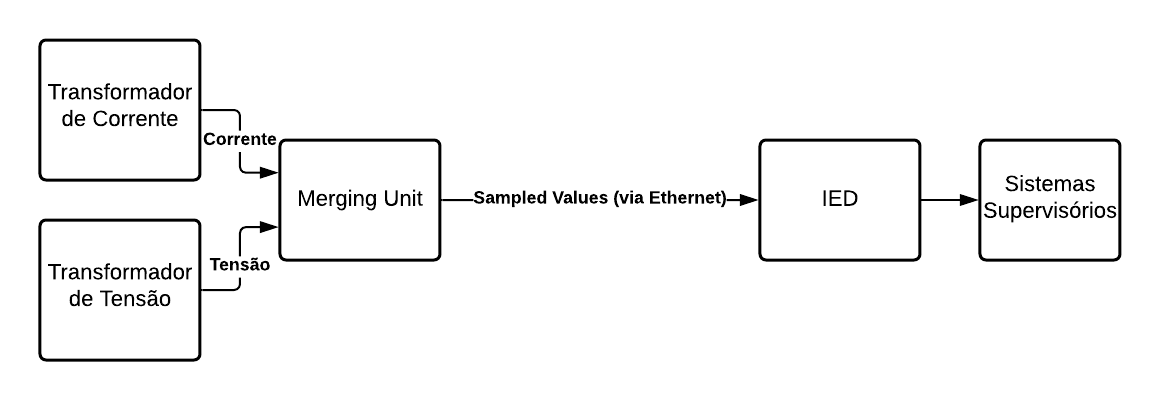
\includegraphics[width=12cm]{pictures/diag_substation_tcc.png}
    \caption{Exemplo de utilização de uma \textit{Merging Unit} em uma subestação elétrica digital}
    \label{fig:diag_substation}
\end{figure}

Neste exemplo, a \textit{Merging Unit} serve como interface entre os transformadores de instrumentação e os IEDs da rede, gerando o fluxo de \textit{Sampled Values} conforme com a norma IEC-61850 \cite{IEC61850_7-2} à partir dos sinais de corrente e tensão aplicados. IED, do inglês \textit{Intelligent Electronic Device} ou Dispositivo Eletrônico Inteligente, é qualquer dispositivo que incorpora um ou mais processadores com a capacidade de receber ou enviar/controlar dados de ou para uma fonte externa de sinal (e.g., relés digitais, disjuntores) \cite{substation_basics}. Já \textit{Sampled Values} \cite{sv_typhoonhil} é o protocolo padrão utilizado para comunicação ente as \textit{Merging Units} e os IEDs. Este protocolo é do tipo \textit{publisher/subscriber}, onde o \textit{publisher} (neste caso a \textit{Merging Unit}), envia mensagens pela rede \textit{Ethernet} periodicamente com intervalos de tempo precisamente definidos. Estas mensagens contém o valor amostrado de cada um dos sinais aplicados nas placas de aquisição analógica da \textit{Merging Unit}. O intervalo de tempo depende de dois fatores: a frequência do sinal medido e a quantidade de amostras por ciclo de sinal. A norma IEC 61850-9-2LE \cite{IEC61850_7-2} define dois valores para a quantidade de amostras por ciclo: 80 para equipamentos de proteção e 256 para equipamentos de medição. Para a frequência do sinal adquirido não há restrições, sendo 50 e 60 Hz os valores mais comumente utilizados. O \textit{subscriber}, representado neste exemplo pelos \textit{IEDs}, ``subscreve'' aos pacotes de \textit{Sampled Values} buscando receber informações sobre um determinado dispositivo da rede.

Para reproduzir esse mesmo ambiente em laboratório, são substituídos os transformadores por uma fonte de tensão e corrente e o IED por um computador, que receberá e processará os \textit{Sampled Values}. A imagem \ref{fig:met_acq} ilustra esse ambiente:

\begin{figure}
    \centering
    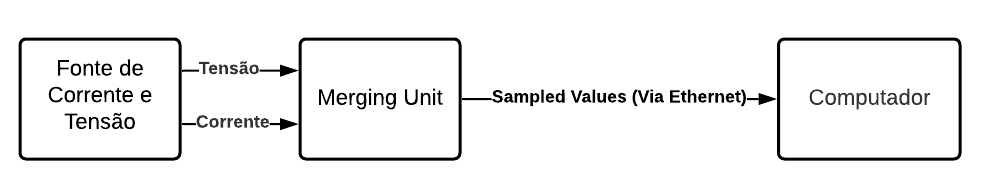
\includegraphics[width=12cm]{pictures/met_acq.png}
    \caption{Ambiente em laboratório para aquisição de dados com \textit{Merging Unit}}
    \label{fig:met_acq}
\end{figure}

Após a aquisição dos \textit{Sampled Values} pelo computador via interface de rede \textit{Ethernet}, se faz necessária a conversão deste fluxo de dados em um formato padrão para oscilografias em sistemas elétricos. Para tanto, é escolhido o formato COMTRADE \cite{comtrade1992} \cite{C37.111-2013}, que é o acrônimo para \textit{Common Format for Transient Data Exchange}, ou Formato Comum para Troca de Dados Transientes. Este formato é composto, no mínimo, por dois arquivos: um arquivo de configuração com extensão .cfg, que descreve os canais de aquisição contidos no COMTRADE e suas características, como frequência nominal do canal, quantidade de canais amostrados, unidade de medição, etc. O quadro \ref{quad:quadro_confcomtra} ilustra um exemplo de arquivo de arquivo de configuração de COMTRADE.

\begin{quadro}[htb]
\caption[Exemplo do arquivo de configuração do COMTRADE]{Exemplo do arquivo de configuração do COMTRADE.}
\label{quad:quadro_confcomtra}
\begin{tabular}{|l|}
%\hline
Test,518,1999 <CR/LF>\\
12,6A,6D <CR/LF>\\
1,P Va-g,,,kV, 0.14462,0.0000000000,0,–2048,2047,2000,1,P <CR/LF>\\
2,P Vc-g,,,kV, 0.14462,0.0000000000,0,–2048,2047,2000,1,P <CR/LF>\\
3,P Vb-g,,,KV, 0.14462,0.0000000000,0,–2048,2047,2000,1,P <CR/LF>\\
4,P Ia,,,A,11.5093049423,0.0000000000,0,–2048,2047,1200,5,P <CR/LF>\\
5,P Ib,,,A,11.5093049423,0.0000000000,0,–2048,2047,1200,5,P <CR/LF>\\
6,P Ic,,,A,11.5093049423,0.0000000000,0,–2048,2047,1200,5,P <CR/LF>\\
1,Va over,,,0 <CR/LF>\\
2,Vb over,,,0 <CR/LF>\\
3,Vc over,,,0 <CR/LF>\\
4,Ia over,,,0 <CR/LF>\\
5,Ib over,,,0 <CR/LF>\\
6,Ic over,,,0 <CR/LF>\\
60 <CR/LF>\\
1 <CR/LF>\\
6000.000,885 <CR/LF>\\
20/07/2005,17:38:26.663700 <CR/LF>\\
20/07/2005,17:38:26.687500 <CR/LF>\\
ASCII <CR/LF>\\
1\\
\hline
\end{tabular}
%\fonte{Teste. -- \showfont}
\end{quadro}

O outro arquivo imprescindível para o COMTRADE é o que contém as próprias amostras, com extensão .dat. Este arquivo pode estar codificado em ASCII com representação decimal separada por vírgulas ou em binário. Os arquivos em ASCII e em binário possuem estrutura idêntica por linha, contendo o número da amostra, o intervalo de tempo em relação ao início do registro em $\mu s$, as medidas analógicas e também as digitais. No modo binário, as informações numéricas estão em formato \textit{little-endian} de 16 bits, enquanto no formato ASCII estas são separadas por vírgula e por uma quebra de linha ao final de cada amostra. O quadro \ref{quad:quadro_dat1comtra} exemplifica essa estrutura.


\begin{quadro}[htb]
\caption[Exemplo de uma linha do arquivo de dados do COMTRADE]{Exemplo de uma linha do arquivo de dados do COMTRADE.}
\label{quad:quadro_dat1comtra}
\centering
\begin{tabular}{|c|}
%\hline
5, 667, –760, 1274, 72, 61, –140, –502,0,0,0,0,1,1 <CR/LF>\\
\hline
\end{tabular}
%\fonte{Teste. -- \showfont}
\end{quadro}


\section{Geração de Sinais e Aquisição pela \textit{Merging Unit}}

%Para capturar os dados necessários para a aplicações dos algoritmos de calibração, se faz necessária a montagem de uma configuração de testes capaz de aplicar sinais previamente programados e com precisão adequada nos canais de tensão e corrente das placas de aquisição analógica da \textit{Merging Unit}. Estes sinais serão condicionados pelo circuito de  instrumentação de entrada da placa e, posteriormente, serão transformados em um fluxo de dados segundo o protocolo \textit{Sampled Values}, conforme a norma IEC-61850 \cite{IEC61850_7-2}, para posteriormente serem capturados por um computador. Este protocolo é usado para a troca de informações entre a \textit{Merging Unit} e os \textit{IEDs - Intelligent Electronic Devices}, ou Dispositivos Eletrônicos Inteligentes, em uma subestação elétrica digital com rede \textit{Ethernet} \cite{sv_typhoonhil}. Um \textit{IED} é qualquer dispositivo que incorpora um ou mais processadores com a capacidade de receber ou enviar/controlar dados de ou para uma fonte externa de sinal (e.g., relés digitais, disjuntores) \cite{substation_basics}.

Na configuração de testes proposta, será utilizada uma fonte de sinais de tensão e corrente programável com precisão maior que as placas de aquisição analógica da \textit{Merging Unit} em análise, de forma a reduzir os erros inerentes ao  sinal aplicado. À partir destes sinais, a \textit{Merging Unit} deverá capturar e processar em tempo real gerando como saída um fluxo de \textit{Sampled Values}. Estes fluxo de dados deverá ser direcionado a um computador para processamento posterior via interface de rede \textit{ethernet}.

\section{Recebimento dos Pacotes de \textit{Sampled Values} e reconstrução dos sinais aplicados}

Já com estes pacotes de \textit{Sampled Values} recebidos pelo computador, é momento de processar esses dados de forma a poder discernir e reconstruir os sinais para cada um dos canais de aquisição analógica da \textit{Merging Unit}. O primeiro passo deste processamento é a conversão desses pacotes em COMTRADEs. Através deste formato, cada uma das amostras presentes nos dados gerados pela \textit{Merging Unit} torna-se um valor numérico de corrente ou tensão, permitindo representar os sinais aplicados pela fonte de tensão e corrente. Na figura \ref{fig:sig_corr_reconst}, é observada essa reconstrução de um sinal de corrente de 50mA RMS:

\begin{figure}[H]
    \centering
    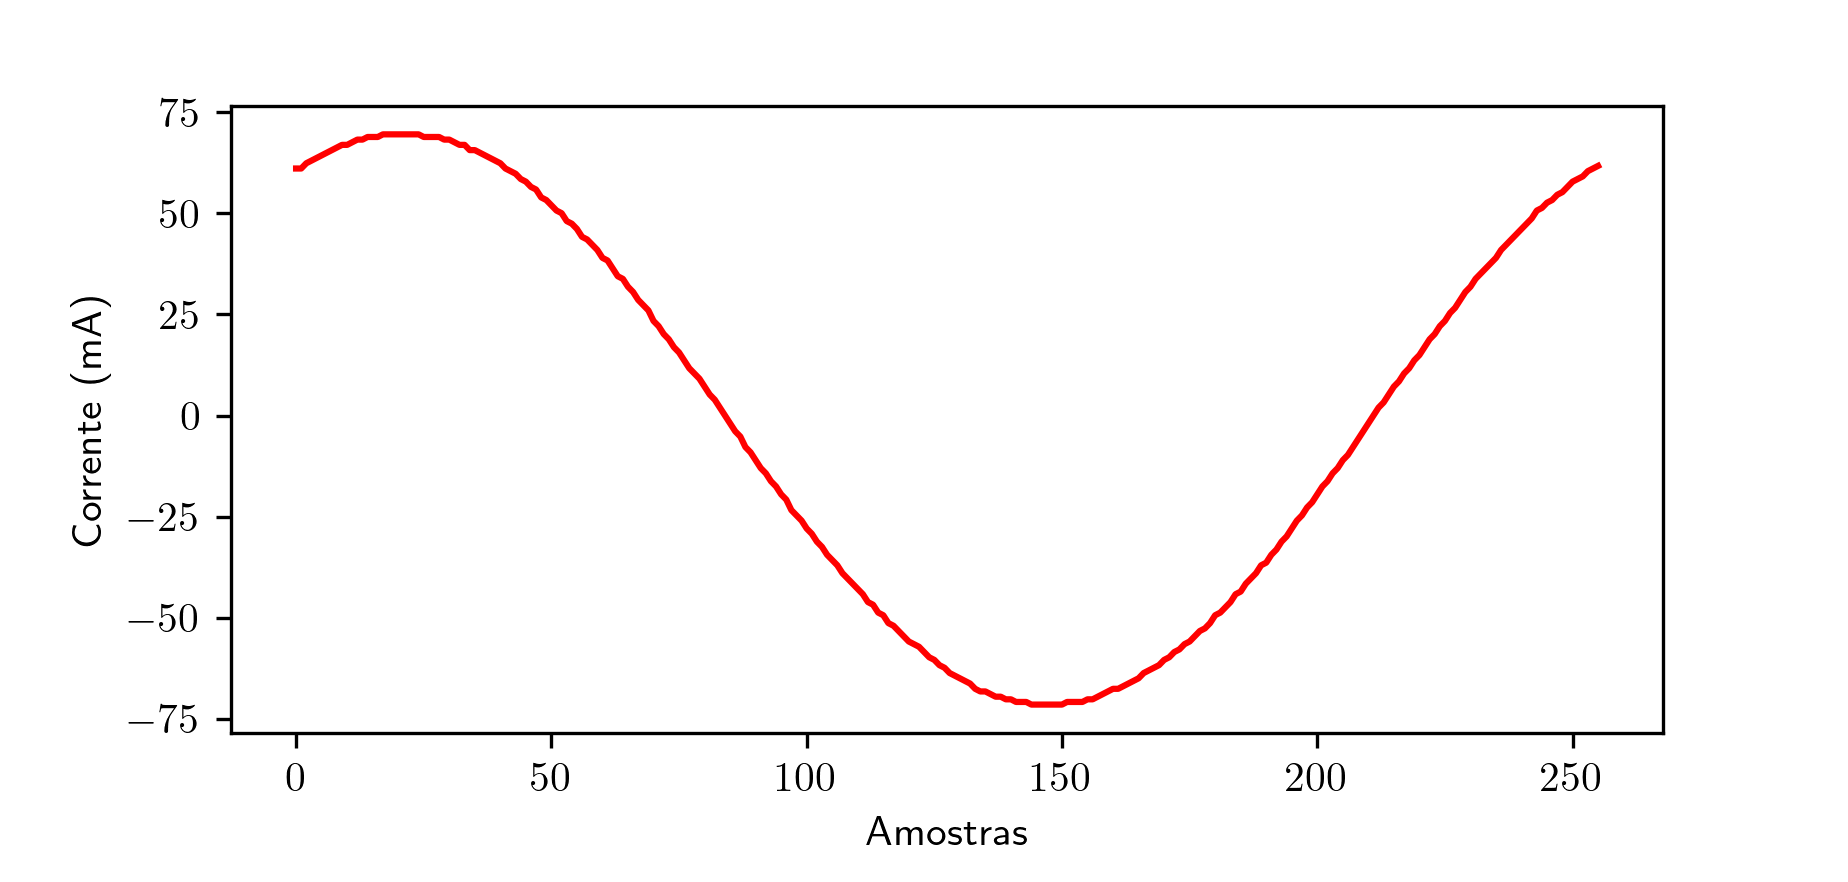
\includegraphics[width=14cm]{pictures/sig_corr_reconst.png}
    \caption{Exemplo de oscilografia construída à partir de COMTRADE.}
    \label{fig:sig_corr_reconst}
\end{figure}

\section{Cálculo dos erros de magnitude e análise da fase e da frequência dos sinais reconstruídos}

Após a reconstrução das amostras para cada um dos canais de aquisição, é calculado o valor quadrático médio ou RMS (do inglês \textit{Root Mean Square}) por ciclo, como exposto na equação \ref{eq:24}:

\begin{equation}\label{eq:24}
RMS(k) = \sqrt{\frac{1}{N} \sum_{i=0}^{N - 1} |u(Nk + i)|^2}
\end{equation} 

Onde N representa o número de amostras por ciclo do sinal avaliado e k é o índice que representa o ciclo atual do sinal. A função $u(Nk + i)$ representa os sinais amostrados de corrente e tensão em análise.

Estes valores são muito informativos pois restringem o múmero de amostras utilizadas como entrada para os algoritmos de calibração de cada canal, sem perder informações substanciais dos sinais originais. 

Neste ponto, é possível calcular os erros de magnitude entre o valor RMS dos sinais aplicados pela fonte e cada um dos valores RMS obtidos por ciclo. De forma a aumentar a variedade dos resultados e trazer mais informações, para cada sinal aplicado são salvos o maior, o menor e a média entre os erros. 

Apesar de não haver sincronismo entre os sinais aplicados pela fonte, isto é, não é sabida a fase inicial destes sinais, é possível ainda assim avaliar eventuais distorções de fase comparando a o sinal obtido à partir do COMTRADE com um sinal senoidal/cossenoidal ideal sem defasamento inicial. Na prática, é possível obter o defasamento inicial através do seguinte procedimento \cite{understandingdsp}: considerando um triângulo retângulo no qual o ângulo será igual ao ângulo de defasamento inicial do sinal, o cateto adjacente será obtido através do produto interno entre as amostras do sinal com fase desconhecida e as amostras do seno ideal, e o cateto oposto será obtido ao efetuar a mesma operação entre as amostras do sinal real e o cosseno ideal. Para conseguir o defasamento, basta obter o arco tangente do quociente entre o resultado dos dois produtos internos. 

Para obter a frequência dos sinais reconstruídos à partir dos COMTRADEs, de forma a poder comparar com a frequência dos sinais gerados pela fonte, é calculada a Transformada Discreta de Fourier (do inglês \textit{Discrete Fourier Transform} ou DFT) do sinal, levando o sinal do domínio do tempo para o domínio da frequência e observando o espectro resultante, onde os pontos diferentes de zero representam as frequências presentes no sinal \cite{lathisig}. O resultado desde procedimento é ilustrado no gráfico da figura \ref{fig:dft_freq}, para um sinal com frequência de 60Hz:

\begin{figure}[H]
    \centering
    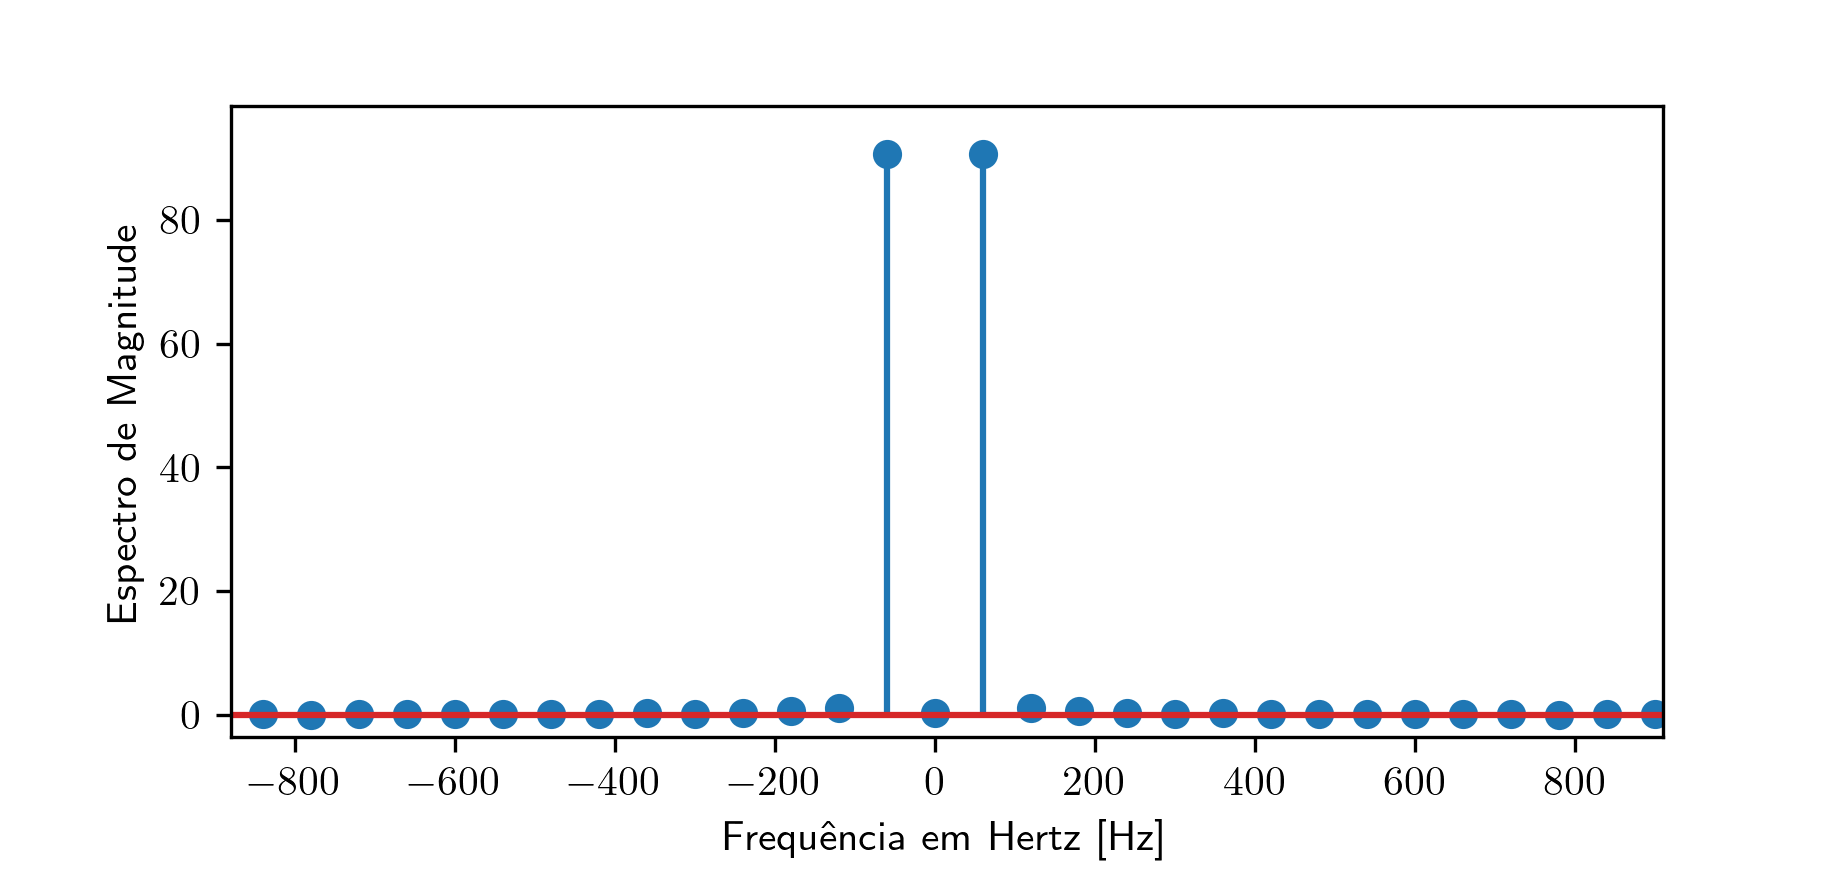
\includegraphics[width=14cm]{pictures/spec_mag.png}
    \caption{Exemplo de espectro de magnitude resultante do cálculo da DFT, a fim de encontrar a frequência do sinal.}
    \label{fig:dft_freq}
\end{figure}

\section{Aplicação dos Métodos de Calibração e avaliação dos Resultados}

Para obter os valores de entrada para os métodos de calibração  descritos no capítulo \ref{cap_algoritmos}, são analisados os valores RMS para cada ciclo de medição e escolhidos os valores que possuam maior erro de magnitude em relação ao valor de referência aplicado pela fonte de tensão e corrente. De forma a ampliar os resultados, também serão utilizados como valores de entrada os valores RMS que possuam o menor erro em relação ao valor de referência e também a média entre os valores RMS de cada ciclo de sinal aplicado.

Com estes valores em mãos, faz-se mister a aplicação destes nos algoritmos, obtendo assim os coeficientes $\alpha$ e $\beta$ de linearização para cada um dos métodos. Estes coeficientes são então aplicados nos valores de entrada, com o intuito de verificar o impacto da calibração dos canais de aquisição sobre os sinais de tensão e corrente amostrados.

A fim de encontrar o melhor entre os algoritmos propostos, são analisados os novos erros de magnitude entre os sinais aplicados pela fonte e os sinais calibrados, bem como figuras de mérito inerentes a este tipo de linearização, como o coeficiente de determinação $R^2$. 

Com o resultado desta análise, é então possível avaliar qual das metodologias de calibração para os canais de aquisição analógica da \textit{Merging Unit} trouxe melhores resultados, isto é: qual reduziu mais os seus erros em relação ao sinal aplicado.

De forma a sumarizar os processos descritos nesta seção, a figura \ref{fig:diag_met_aval} ilustra cada um dos passos acima descritos.

\begin{figure}[H]
    \centering
    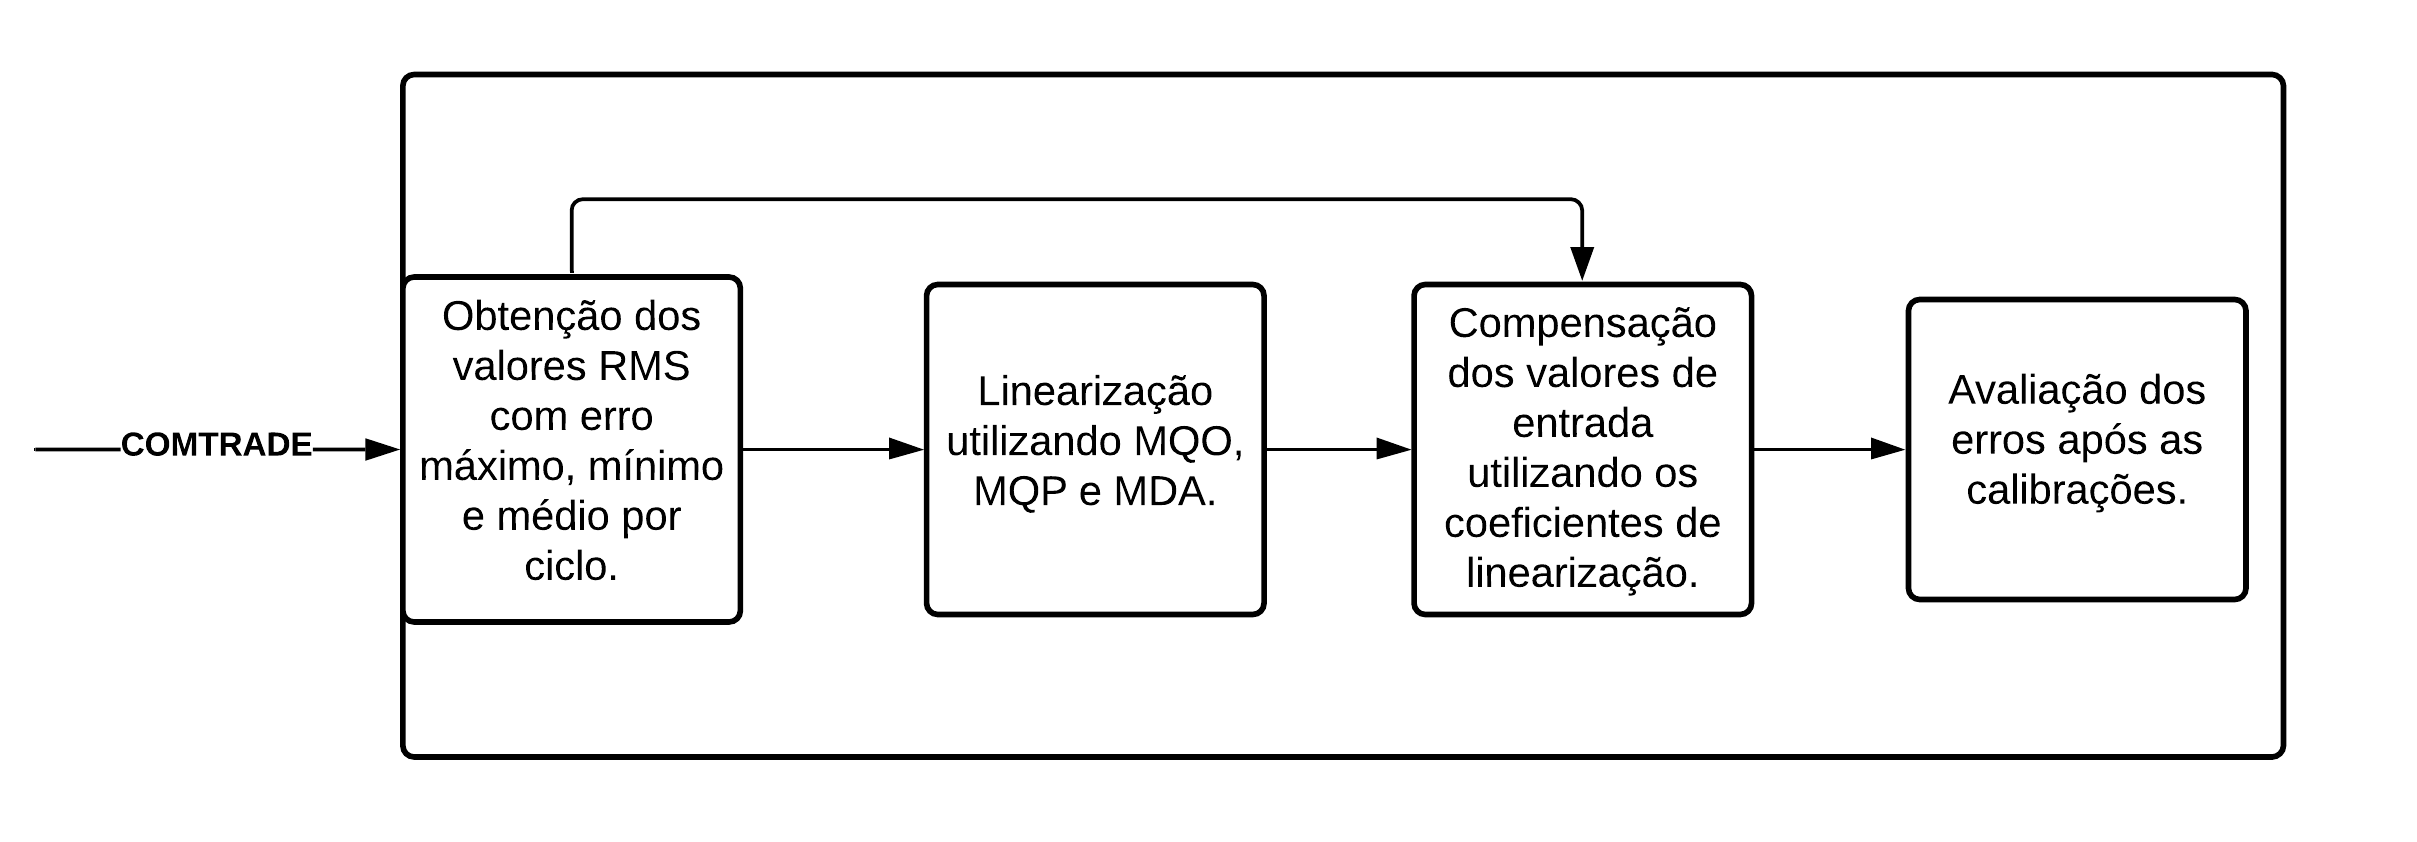
\includegraphics[width=14cm]{pictures/diag_met_avalia.png}
    \caption{Diagrama dos procedimentos descritos na seção de aplicação dos métodos de calibração e avalia os resultados.}
    \label{fig:diag_met_aval}
\end{figure}

\end{otherlanguage*}

